\documentclass{beamer}
\usepackage{pgfpages}
\setbeamertemplate{note page}[plain]
\setbeameroption{show notes on second screen}
\usepackage[ngerman]{babel}
\usepackage{booktabs}
\usepackage{tabulary}
\usepackage{siunitx}
\usetheme{imise}
\author[Sebastian Stäubert]{Konrad Höffner, Franziska Jahn, Christian Kücherer, Barbara Paech, Birgit Schneider, Martin Schöbel, \textbf{Sebastian Stäubert}, Alfred Winter}
\date[20.9.2017 10:15]{Mittwoch 20. September 2017, 10:15--10:30 Uhr\\
GMDS Jahrestagung, Raum A01 0-006}
\title{Technische Umgebung der SNIK Ontologie\\~}
%\institute{GMDS Jahrestagung 2017}
\subtitle{Ein Semantisches Netz des Informationsmanagements im Krankenhaus}
\newcommand{\todo}[1]{TODO: #1}
\newcommand{\imageslide}[4][]
{
\begin{frame}{#2}
\centering\includegraphics[width=1\textwidth,height=0.8\textheight,keepaspectratio]{#3}
\\#1
\note{#4}
\end{frame}
}

\begin{document}
\begin{frame}
\titlepage
\end{frame}


\imageslide[\url{http://www.snik.eu} \url{http://5stardata.info}]{SNIK Projekt}{img/5star.png}
{
\begin{itemize}
\item kurze Einführung SNIK-Projekt
\item offene Bereitstellung von computerverarbeitbaren Fakten des Informationsmanagements im Krankenhaus aus Lehrbüchern
\item Nutzen maximieren: 5 Sterne Schema für offene Daten von Tim Berners-Lee
\end{itemize}

\begin{enumerate}
\item Rechtssicherheit für Benutzer durch offnene Datenlizenz. PDFs der Bücher dürfen allerdings nicht online gestellt werden. Nur wenn jemand fragt:
\begin{itemize}
\item CC BY-NC-SA 4.0 Lizenz (Creative Commons Attribution-NonCommercial-ShareAlike).
\item Erlaubt: Teilen, Adaptieren
\item Bedingungen: Attribution, Nichtkommerziell, gleiche Lizenz für Derivate. Für eine offene Lizenz recht restriktiv, sind aber für andere Optionen offen
\end{itemize}
\item Strukturiertes Format: Lesen der Bücher und manuelles modellieren der Fakten in Tabellen, sehr zeitaufwändig 
\item Stufe 3 trivial: speichern in offenem Format, in unserem Fall CSV
\item Konvertierung der Tabelle zu einer Ontologie mittels Tarql scripts, viel Vorarbeit in Tabellen 
\item Interlinks zwischen Büchern automatisch erstellt durch LIMES
\end{enumerate}

}
\begin{frame}{Einsatz}
\centering
\begin{tabular}{ll}
\toprule
\textbf{Ziel}	&\textbf{Zielgruppe}\\
\midrule
Lehre			&Lehrer und Studenten\\ 
Datenintegration	&Krankenhausleitung, CIO\\
Formalisierung		&Domänenexperten, Ontologen\\
\bottomrule
\end{tabular}
\end{frame}

\begin{frame}{Ziele}
\begin{enumerate}
\item Publizieren 
\item Visualisieren 
\item Evaluieren
\item Integrieren 
\end{enumerate}
\end{frame}


\imageslide[\url{https://github.com/IMISE/snik-ontology}]{RDF Dump}{img/rdfdump.png}{}
\imageslide[\url{https://protegewiki.stanford.edu/}]{RDF Dump in Protégé}{img/protege.png}{}
\imageslide[\url{http://www.snik.eu/sparql}]{SPARQL Endpoint}{img/sparqlresult.png}{}

\imageslide[\url{http://www.snik.eu/ontology}]{RDF Browser---LodView}{img/browse-cio.png}{}

\imageslide[\url{http://www.snik.eu/graph}]{Graphvisualisierung I}{img/graph-entitytype.png}{}
\imageslide[\url{http://www.snik.eu/graph}]{Graphvisualisierung II}{img/graph-erf.png}{}
\imageslide[\url{http://www.snik.eu/graph}]{Graphvisualisierung---Kürzester Weg}{img/shortestpath.png}{}
\imageslide[\url{http://www.snik.eu/graph}]{Graphvisualisierung---Spiderworm}{img/spiderworm.png}{}

\begin{frame}{LodLive \& Relfinder}
\centering
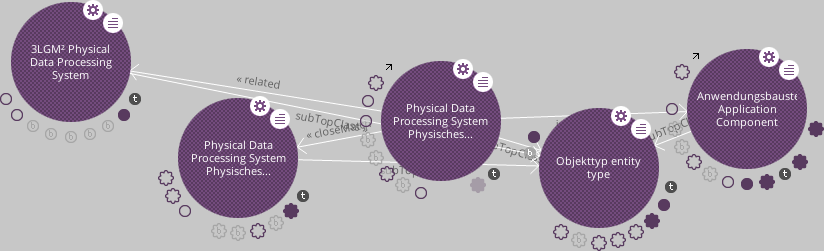
\includegraphics[width=\textwidth]{img/lodlive.png}\\
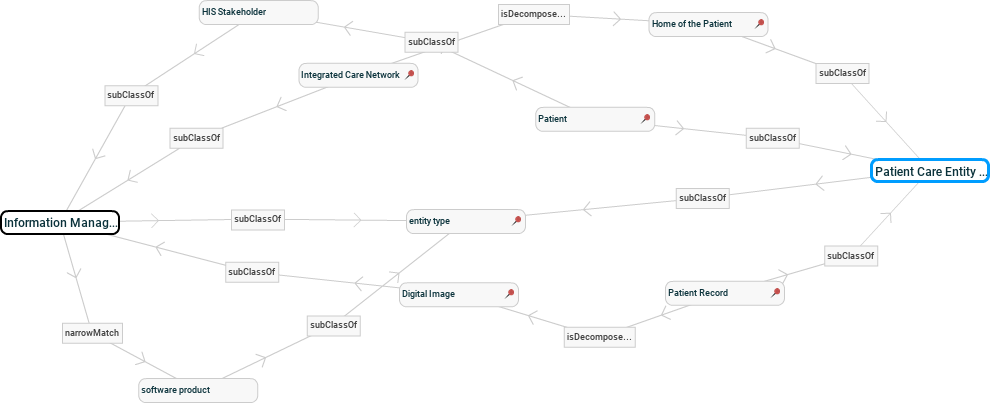
\includegraphics[width=\textwidth]{img/relfinder.png}
\end{frame}



\imageslide[https://imise.github.io/snik-ontology/2017/04/12/dashboard]{Statistiken}{img/dashboard-medley.png}{}
\imageslide[\url{https://github.com/IMISE/snik-ontology/issues}]{Ticketsystem}{img/gitissue.png}{}
\imageslide[\url{http://www.snik.eu/evaluation}]{TripleCheckMate}{img/triplecheckmate.png}{}



\imageslide[\url{http://www.snik.eu/sparql}]{SPARQL Endpoint}{img/sparqlresult.png}{}

\imageslide[http://aksw.org/Projects/LIMES]{LIMES}{img/limes.png}{}

\iffalse
\begin{frame}{Interlinking}
\begin{itemize}
\item Verknüpfungen zwischen Klassen verschiedener Ontologien
\item LIMES Tool von AKSW um Axel Ngonga
\item Finden von Kandidaten durch Stringähnlichkeit, manuelle Verifizierung und Kategorisierung
\end{itemize}
\end{frame}
\fi

\imageslide[https://github.com/IMISE]{Öffentliche Softwarerepositories}{img/github.png}{}



\begin{frame}
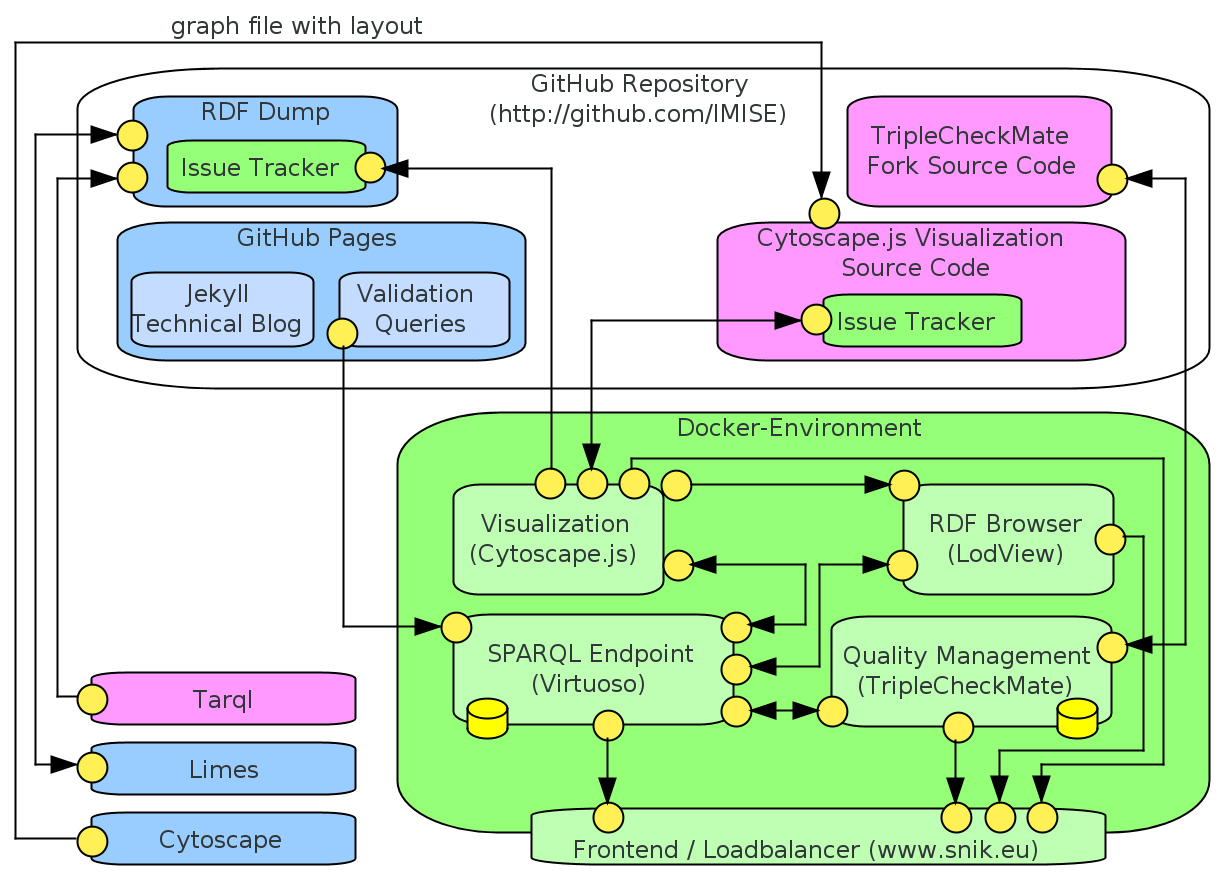
\includegraphics[width=\textwidth]{img/architecture.png}
\end{frame}

\begin{frame}[fragile]{Fragen?}
\begin{itemize}
\item Diese Präsentation \url{https://github.com/KonradHoeffner/latex/releases/download/colloquium/colloquium.pdf}
\vspace{0.5em}%here it works as intended
\item Überblick \url{http://www.snik.eu}
\item Visualisierung \url{http://www.snik.eu/graph}
\item SPARQL Endpunkt \url{http://www.snik.eu/sparql}
\item RDF Browser \url{http://www.snik.eu/ontology}
\item Evaluation \url{http://www.snik.eu/evaluation}
\item Twitter \url{https://twitter.com/snik\_proj}
\item Technisches Blog \url{https://imise.github.io/snik-ontology}
\item GitHub Organisation mit Ticketsystem \url{https://github.com/imise}
\end{itemize}
\end{frame}

\begin{frame}[fragile]{Externe Tools und Bibliotheken}
\begin{itemize}
\item LIMES Interlinker \url{http://aksw.org/Projects/LIMES}
\item Tarql Konvertierungstool \url{https://tarql.github.io/}
\item Cytoscape.js Graphbibliothek \url{http://js.cytoscape.org/}
\item Cytoscape Desktopvisualisierung \url{http://www.cytoscape.org/}
\end{itemize}
\end{frame}
 
\end{document}
